\section{Execise Integration}\label{5_2_gestureConstruction}
%- Recording of gestures --> Kinectstudio --> Making/Train gestures --> Visual gestures builder
The system should guide the user through predefined exercises for learning slacklining. To give feedback in an appropriate manner the exercises are recorded as custom gestures. The \textit{Kinect for Windows Human Interface Guidelines} describe the term \textit{gesture} as follows: "[...] we use the term gesture broadly to mean any form of movement that can be used as an input or interaction to control or influence an application."~\cite{MicrosoftHIG2014-mh}.
There are two approaches of creating custom gestures. The first is one is to do heuristics, which means to manually track the position of each joint and write conditions according to the action that should happen if the joints exceed a threshold or are is in a defined range. This is used and implemented for simple gestures like raising the hand over the head. For more complex gestures, the developer must have a good understanding about how the human body behaves and moves. In the most cases developer have not the appropriate expertise. Hence it is recommended to use the Visual gesture builder (VGB) provided by Microsoft for more complex gestures.
%any form of movement that can be used as an input or interaction to control or influence an application. Gestures can take many forms, from simply using your hand to target something on the screen, to specific, learned patterns of movement, to long stretches of continuous movement using the whole body.

\subsection{Visual gesture builder}
This tool relies on machine learning and looks at the data given by the developer via pre recorded clips. With these it builds a database that can then be used to track the actual gesture in an application. The more data is provided to it the better the detection by the Kinect. Another advantage is that environmental factors are not that complex to handle as in comparison to heuristics. For example if the sensor is set too high or too low the developer has to consider this in his code and it can blow up managing and maintaining such factors in code. With the VGB the developer just records data with the sensor on the appropriate height and let the machine learning algorithm learn it. The cons are the huge file size of the recorded clips which can take very much disk space. Also setting the keyframes for parts that the builder should detect is time consuming whereas on the other hand it is simple and user friendly.

\subsection{Building gestures workflow}
The workflow for creating a gesture is almost always the same (Figure~\ref{fig:5_3_gestureCreation}). 
First the actual gesture has to be recorded via KinectStudio. This is a tool provided by Microsoft for monitoring and recording clips of the Kinect streams. After finishing with the recording a new project can be made in the Visual Gesture Builder. The developer selects the body parts that are necessary for the gesture. After that the indicator of the gesture has to be defined, i.e. if it is discrete or continuous. Discrete means that the system determines if a gesture is currently performed or not. It provides a confidence value that determines the correctness of the persons execution regarding the specific gesture. This is the majority for gesture tracking like e.g. raising the hand or lifting a leg. However the continuous indicator means that the progress of a gesture can be measured. Often multiple small gesture are combined to an entire gesture. This could be for example a golf swing or switching the standing leg, where rather the progress has to be measured than the confidence~\cite{MicrosoftVGB}.

\begin{figure}[htb]
	\centering
	\begin{minipage}[t]{1\linewidth}
		\centering
		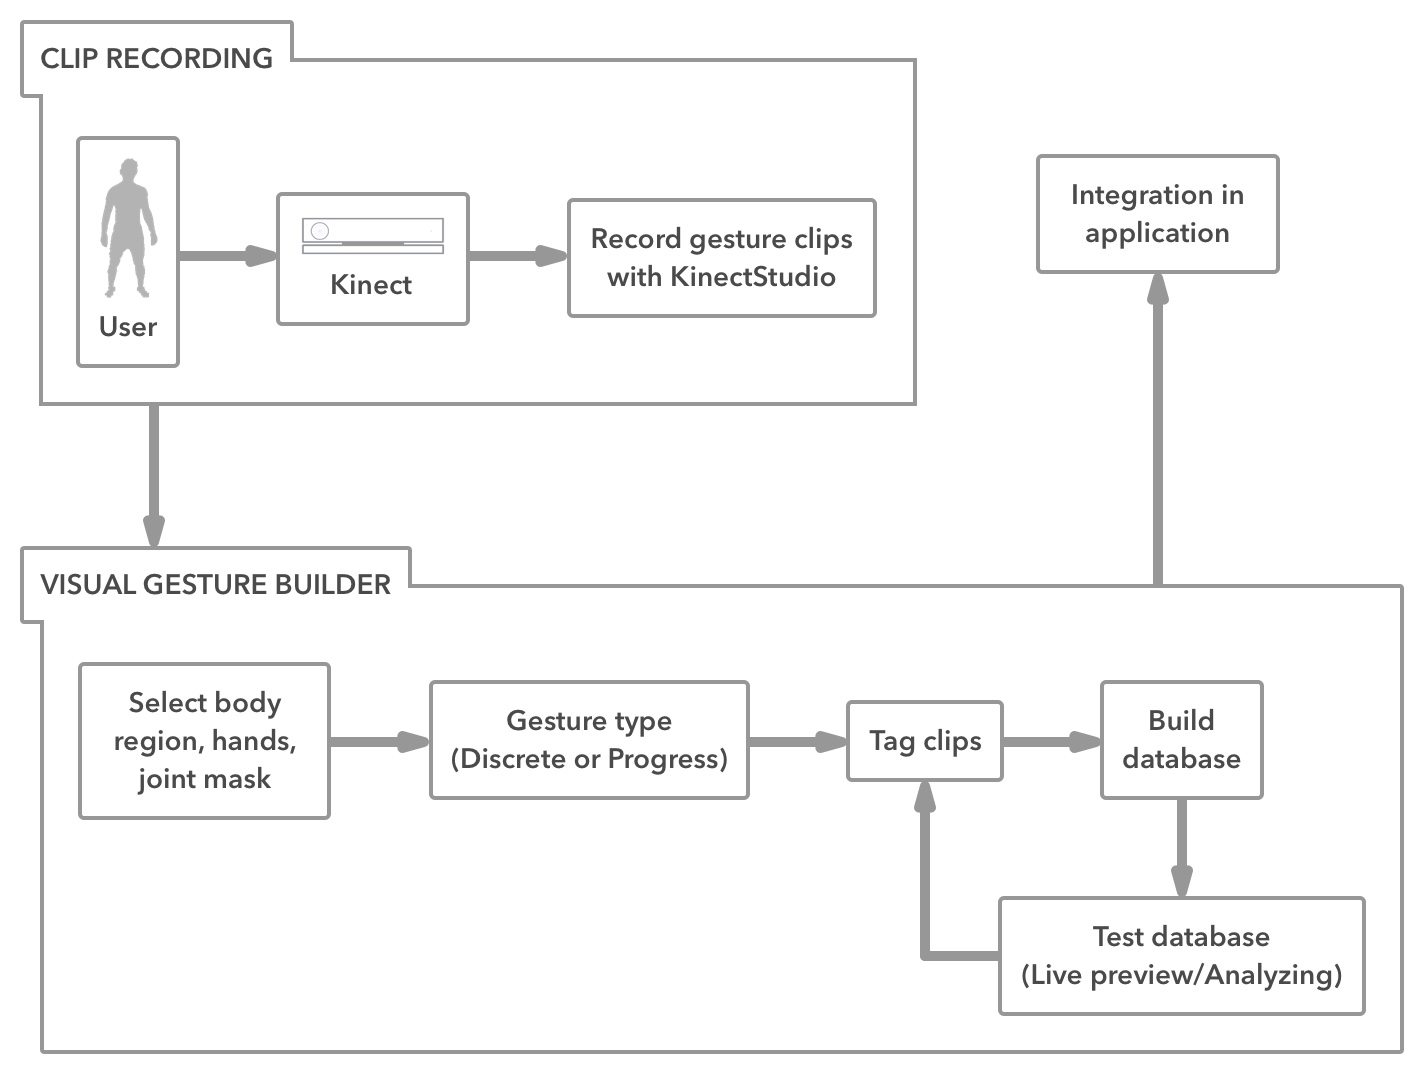
\includegraphics[width=1\linewidth]{Pictures/5_3_gestureCreation}
		\caption{Workflow of creating a gesture database}
		\label{fig:5_3_gestureCreation}
	\end{minipage}
\end{figure}

After the project creation training data can be inserted, which are the prior recorded clips. The developer has to define tags that describe the starting and the end point of the gesture. After finishing with the tagging a gesture database file can be built. Afterwards it can be analysed via a live preview or with other recorded clips in a separate analysing area. If some misbehaviour appears the developer has to record and add more clips for the gesture or the tags have to be adjusted. Lastly after the testing phase a gesture database file can be built and then implemented in the application for gesture detecting. %The structuring of the application architecture is part of the next section.